\section{Jonas}
%================================ FRAME 1 ================================
\subsection{Overview}
\begin{frame}{Jonas: Overview}
\begin{itemize}
	\item Introduction:
  		\begin{itemize}
			\item What is GIRAF?
			\item Project Focus
		\end{itemize}
	\item Project Organization:
		\begin{itemize}
			\item Development Methods
			\item Inter-Group Communication
		\end{itemize}
\end{itemize}
\end{frame}
 
%================================ FRAME 2 ================================
\subsection{Project Basics}
\begin{frame}{What is GIRAF?}
\begin{itemize}
	\item Suite of Android Applications
		\begin{itemize}
		    \item Assisting citizens with autism 
  			\item Learning and Planning
  			\item Ongoing since 2011
		\end{itemize}
	\item Multi-Project
		\begin{itemize}
		    \item Collaborative Development 
  			\item Code Maintainence
		\end{itemize}
\end{itemize}
\end{frame}

%================================ FRAME 2 ================================
% \begin{frame}{GIRAF Applications}
% 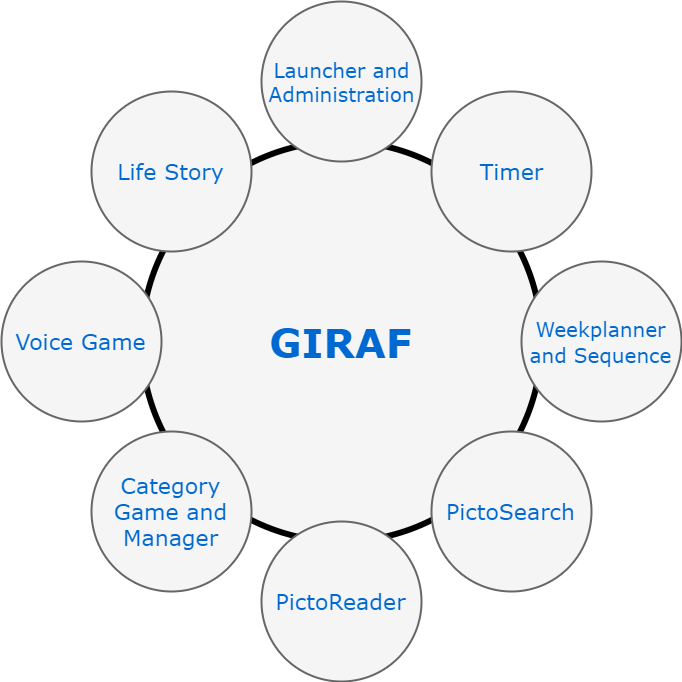
\includegraphics[scale=0.32]{figures/GirafApps.png} 
% \end{frame}

%================================ FRAME 3 ================================
% \begin{frame}{Original State of Giraf}
% \begin{itemize}
% 	\item Front End
% 		\begin{itemize}
% 		    \item Mostly Finished
%   			\item User Testing
%   			\item Occasionally Questionable Design
% 		\end{itemize}
% 	\item Back End
% 		\begin{itemize}
% 		    \item Incomplete
% 		    \item Questionable Quality
% 		    \item Lack of Flexible Database Communication
% 		\end{itemize}
% \end{itemize}
% \end{frame}
% 
% %================================ FRAME 3 ================================
% \begin{frame}{Project Focus}
% \begin{itemize}
% 	\item Finalize Selected Applications
% 	\item Make Changes From User Feedback
% 	\item Implement Usable Database Communication
% \end{itemize}
% \end{frame}

%================================ FRAME 2 ================================
\begin{frame}{Project Focus}
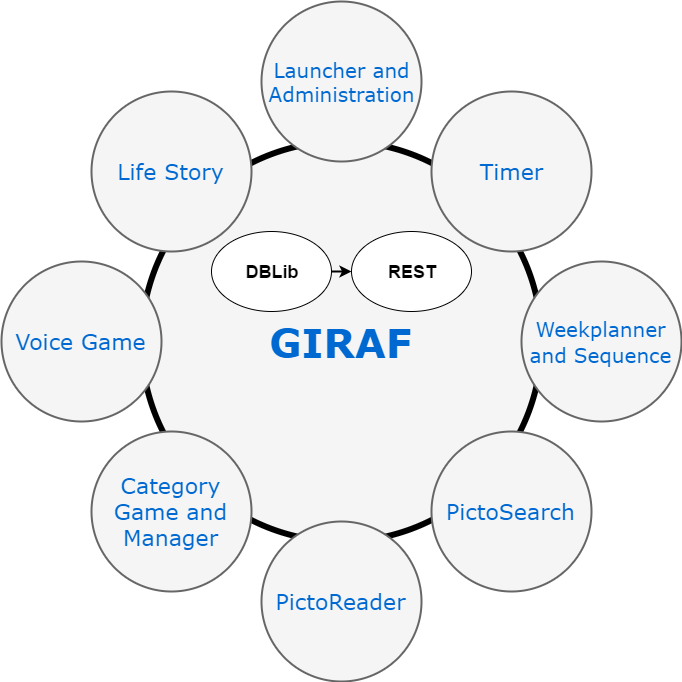
\includegraphics[scale=0.32]{figures/GirafFocus.png} 
\end{frame}

%================================ FRAME 2 ================================
\begin{frame}{Our Group's Focus: Login}
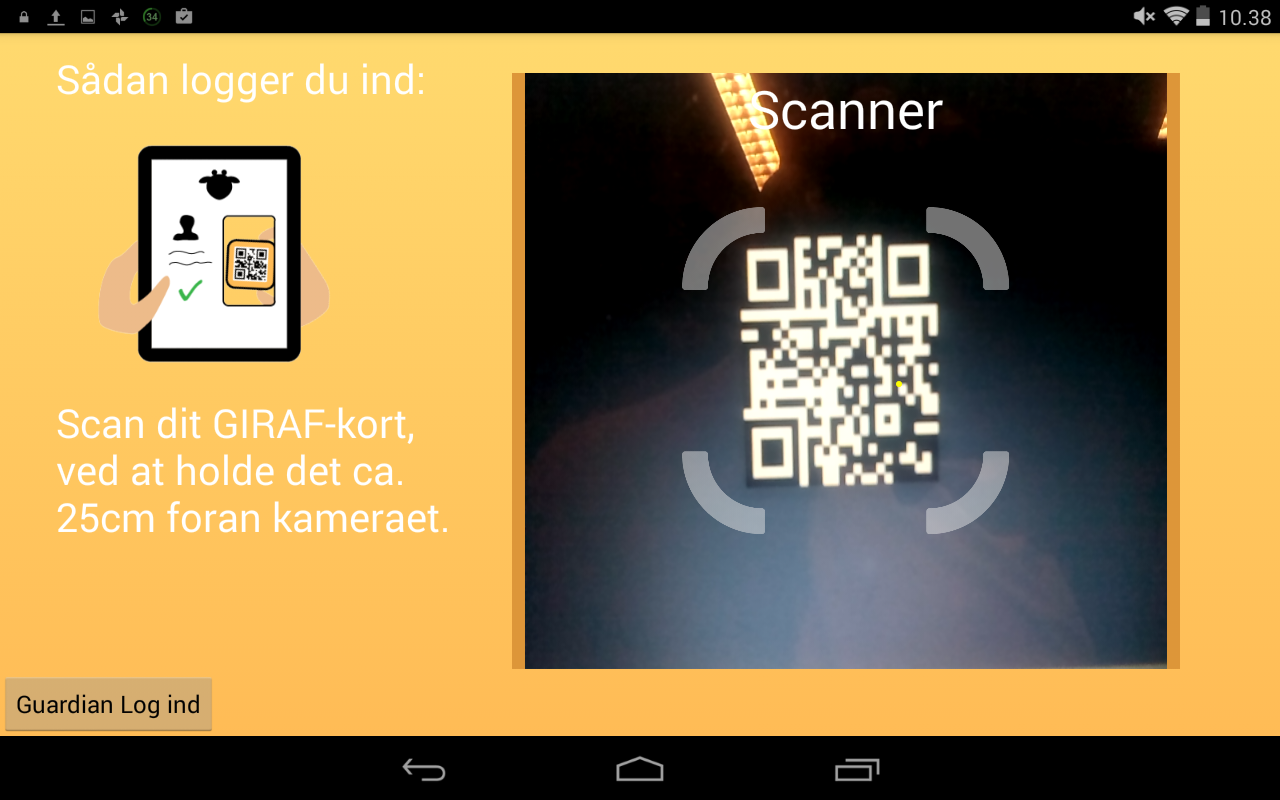
\includegraphics[scale=0.21]{figures/Login.png} 
\end{frame}

%================================ FRAME 2 ================================
\begin{frame}{Our Group's Focus: Main Screen}
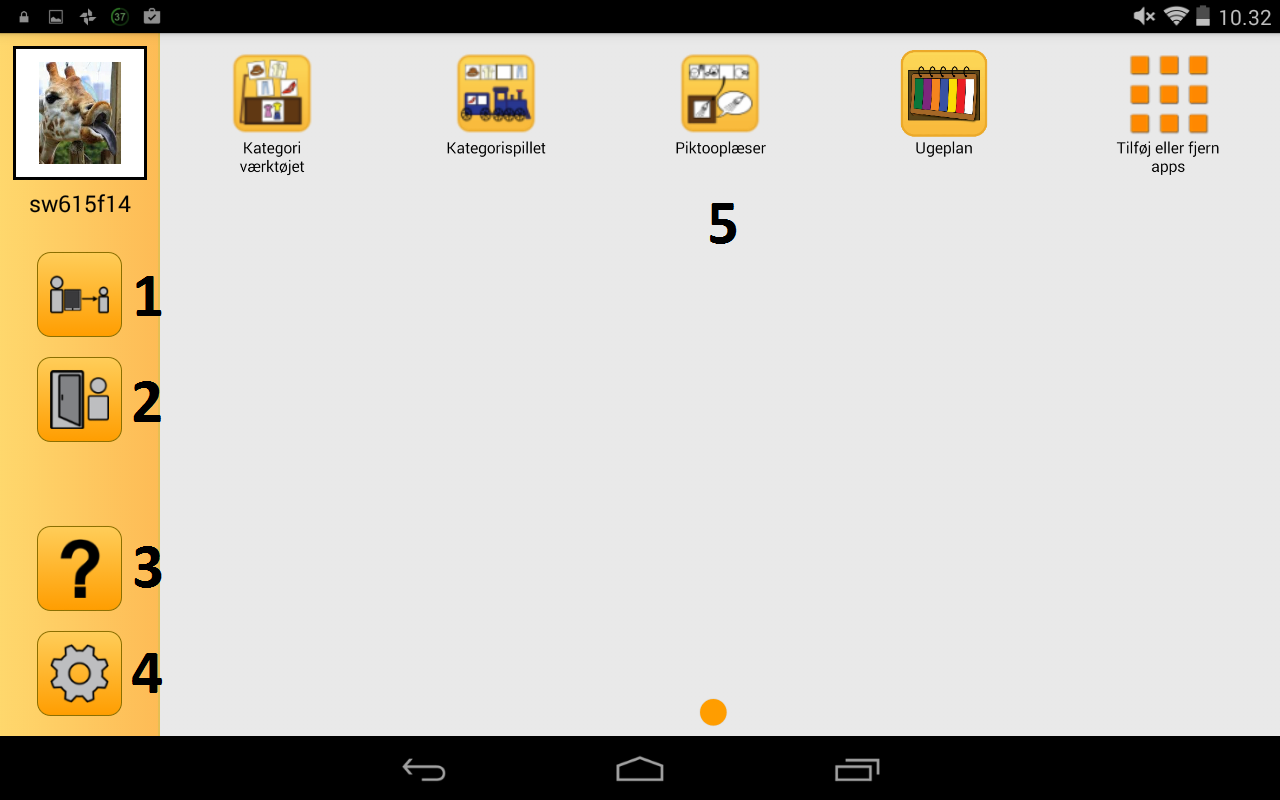
\includegraphics[scale=0.28]{figures/MenuGuardian.png} 
\end{frame}

%================================ FRAME 4 ================================
\subsection{Project Organization}
\begin{frame}{SCRUM of SCRUMS}
\begin{itemize} 
	\item Each Group Organizes Their Own SCRUM
	\item Representative SCRUM Group
	\item Reflection
\end{itemize}
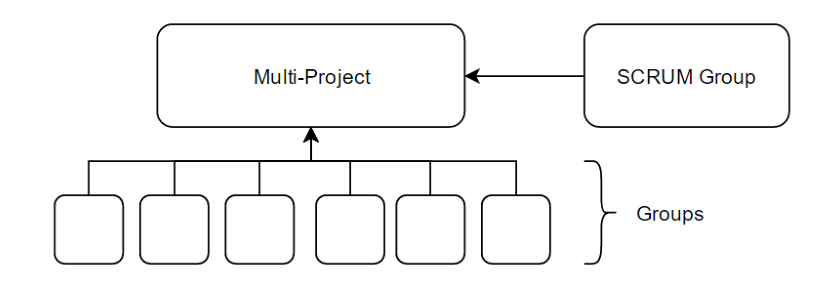
\includegraphics[scale=0.42]{figures/SoS.png} 
\end{frame}

%================================ FRAME 4 ================================
\begin{frame}{Master SCRUM}
\begin{itemize} 
	\item Present weekly work, and what to do
    \item What problems do we have
    \item Knowledge Sharing
    \item Reflection
\end{itemize}
\end{frame}

%================================ FRAME 4 ================================
\begin{frame}{Sprint Meetings}
\begin{itemize} 
	\item PO presented user stories
    \item Developers split into groups to brainstorm tasks
	\item Reflection
\end{itemize}
\end{frame}

%================================ FRAME 4 ================================
\begin{frame}{Communiaction}
\begin{itemize} 
	\item Shared Chat Rooms
	\item Close Proximity
	\item Dynamically Planned Meetings
	\item Reflection
\end{itemize}
\end{frame}
